\documentclass[a4paper,11pt]{article}
\usepackage[T1]{fontenc}
\usepackage[utf8]{inputenc}
\usepackage{lmodern}
\usepackage[italian]{babel}
\usepackage{minted}
\usepackage{pgffor}
\usepackage{graphicx}
\usepackage{subfig}
\usepackage{amsmath}
\usepackage{tabularx}
\usepackage[bookmarks,hidelinks]{hyperref}
\usepackage[style=numeric-comp,hyperref,useprefix,backend=bibtex]{biblatex}
\bibliography{biblio.bib}
\title{Progetto di sistemi complessi: modelli e simulazione}
\author{Pietro Brenna (781840) \\ Alessandro Bregoli (780711)}
\date{}
\begin{document}

\maketitle
\newpage
\tableofcontents
\newpage

\section{Introduzione}
  
La modellazione ad agenti è senza dubbio un metodo valido per simulare l'esplorazione
di uno spazio da parte di robot; ciò che distingue i vari approcci studiati è 
l'architettura dell'agente-robot, i metodi di interazione, il modello decisionale.

Nei modelli esistenti si cerca l'ottimalità dell'esplorazione (come tempo, come lunghezza dei percorsi), ed emergono due approcci fondamentali:
\begin{itemize}
	\item Un solo robot costoso (computazionalmente) che ricerca cerca di approssimare l'esplorazione ottimale
	\item Diversi robot poco costosi coordinati da un nodo centrale (costoso computazionalmente)
\end{itemize}
Entrambi gli approcci soffrono di una caratteristica indesiderabile: hanno un single point of failure che rende inutilizzabile l'intero modello.

Il nostro lavoro rinuncia all'ottimalità dell'esplorazione: accontentandosi di un comportamento "buono" anche se non ottimale, è possibile eliminare il coordinamento centrale, mantenere i vari robot poco costosi e ottenere robustezza di comportamento.

\newpage
\section{Stato dell'arte}
  Nel campo dell'esplorazione multi-robotica si trovano in letteratura approcci
diversi che coprono problematiche simili. 
Troviamo ad esempio \cite{gerkey2004formal} guarda al modello
decisionale degli agenti sotto l'aspetto della task allocation, approccio da cui abbiamo tratto spunto per il nostro lavoro.
Non mancano tuttavia esempi di modelli, come in \cite{bourgault2002information},
che analizzano il problema con gli strumenti della teoria dell'informazione;
tale lavoro dà anche soluzione al problema di navigazione, stabilire la propria
posizione nell'ambiente, mentre in \cite{dudek1996taxonomy} si guarda al
problema da tutt'altra prospettiva ed il solo posizionamento relativo tra robot
vicini viene usato per condurre a termine l'esplorazione.

Vale la pena sottolineare che nel nostro lavoro non ci occupiamo della
navigazione e la posizione assoluta degli agenti sulla griglia è sempre nota con
precisione.

\cite{gerkey2004formal} Sviluppando un sistema composto da robot multipli che devono cooperare 
una delle domande chiave è: "quale robot deve eseguire che task?"; 
a questa domanda tenta di rispondere la branca della ricerca che
si occupa di multi-robot task allocation (MRTA).
Per task si intende un sottogoal necessario per ottenere l'obiettivo generale.

\subsection{Funzione da ottimizzare}
  Per trattare MRTA in un contesto di ottimiziazione è necessario decidere cosa deve essere
  ottimizzato. Idealmente il goal è di ottimizzare le performance del sistema, ma questo valore
  è spesso difficile da misurare durante l'esecuzione del sistema.
  Inoltre, quando si sceglie tra diverse possibilità, l'impatto sulle performance del sistema di ogni opzione
  solitamente non è conosciuto; quindi è necessario una stima delle performance. Viene dunque introdotto
  il concetto di "utility" definito come quel valore che:
  \begin{enumerate}
    \item Rappresenta la qualità dell'esecuzione del compito assegnato dati il
          metodo e l'equipaggiamento.
    \item Rappresenta il costo in risorse dati i requisiti spazio-temporali del
          lavoro assegnato.
  \end{enumerate}
  
\subsection{Un approccio collaborativo}
  \cite{burgard2002collaborative} L'obiettivo di un processo di esplorazione è quello di esplorare l'intero ambiente 
  nel minor tempo possibile. Questo modello utilizza un ambiente discretizzato attraverso una griglia. Durante la 
  scelta degli obiettivi per i robot vengono tenunte in considerazione le celle di frontiera (celle esplorate con
  almeno un vicino non esplorato) e si calcola una funzione di costo che è inversamente proporzionale alla distanza
  dal robot per cui si sta cercando l'obiettivo e direttamente proporzionale al numero di robot che si stanno diriginedo
  verso quella cella. Un altro dato da considerare è l'utilità di una cella di frontiera. Tale valore è
  difficile da calcolare tuttavia possiamo aspettarci che una cella obiettivo di un robot avrà un valore di utilità
  inferiore per gli altri. \\
  La selezione del target appropriato per ogni robot tiene in considerazione il costo dello spostamento verso il target
  e l'utilità della cella target. In particolare per ogni robot $i$ cerchiamo un compromesso tra il costo $V^i_t$ di
  muoversi verso la cella $t$ e l'utilità $U_t$ di $t$.
\subsection{Complessità delle mappe}
  Sono state sviluppate diverse metriche per caratterizzare la "difficoltà" di
  una mappa; la maggior parte degli approcci in letteratura si dedicano al
  problema affine di calcolare la difficoltà di un labirinto con una uscita e un
  ingresso; per dare una soluzione elegante a tale problema ad esempio,
  \cite{amancio2011concepts} e \cite{mcclendon2001complexity} si basano su una
  rappresentazione a grafo dell'ambiente e ne calcolano le proprietà; in più
  in \cite{amancio2011concepts} si fa riferimento all'``absorption time'', ovvero
  la probabilità che un cammino randomico arrivi dall'entrata all'uscita.
  Tuttavia per il nostro approccio non è sufficiente considerare la mappa un
  labirinto.
\subsection{Legge di Amdhal}
  La legge di Amdhal\cite{amdhal} in informatica è quella formula che rappresenta 
  l'aumento teorico di velocità di esecuzione derivante da una 
  parallelizzazione del problema. 
  $$S_{lantency}(s) = \frac{1}{(1-p) + \frac{p}{s}}$$
  dove:
  \begin{itemize}
    \item $S_{lantency}$: é il guadagno teorico di performance dell'intero task
    \item $s$: è il fattore che rappresenta le risorse del sistema
    \item $p$: rappresenta la proporzione tra la parte di sitema parallelizzabile e quelle non parallelizzabile
  \end{itemize}
  
  $$\begin{cases}
    S_{latency}(s) \leq \frac{1}{1 - p} \\
    \lim\limits_{s \to \infty} S_{latency}(s) = \frac{1}{1 - p}.
    \end{cases}$$
  Da questo possiamo evincere che aumentando all'infinito le risorse di parallelizzazione il sistema raggiungerà un minimo rappresentato
  dalla sua parte non parallelizzabile.
  Una possibile derivazione di questa formula è l'equazione che ricava il
  tempo teorico di esecuzione del sistema:
  $$T(s) = (1-p)T + \frac{p}{s}T$$
  
  

\newpage
\section{Modello}
  Il modello che andremo a presentare si prefigge lo scopo di esplorare un territorio
in cui possono esserci degli ostacoli insormontabili. Si tratta di un modello distribuito; in questo modo
si può contrastare il problema del single point of failure; tuttavia per poter
sopperire a questo problema ogni robot deve possedere una certa capacità computazionale ed
una buona capacità comunicativa. Questi robot dovranno dunque essere in grado di comunicare tra loro; dovranno
inoltre essere in grado di selezionare obiettivi e percorsi; in fine dovranno avere modo di salvare la mappa.\\
Il modello è scalabile ma bisogna tenere in considerazione la quantità di dati che vengono scambiati tra i robot
all'aumentare degli stessi.
\subsection{Classificazione in quanto sistema di robot}
Secondo la tassonomia di Dudek et al \cite{dudek1996taxonomy} il nostro modello
ricade nelle categorie:
\begin{itemize}
	\item per quantità, SIZE-LIM: i robot sono pochi rispetto alla dimensione
	      dell'ambiente
	\item per raggio di comunicazione, COM-INF: ogni robot può comunicare con
	      qualsiasi altro robot.
	\item per topologia di comunicazione, TOP-BROAD: ogni messaggio è ricevuto
	      da ogni robot (broadcast)
	\item per banda di comunicazione, BAND-INF: non modelliamo il costo delle
	      comunicazioni, anche se vedremo che si ricava facilmente un limite
	      superiore
	\item per flessibilità di riposizionamento, ARR-DYN: ogni robot si muove
	      indipendentemente dai movimenti degli altri robot.
	\item per potenza elaborativa, PROC-TME: il calcolo del goal richiede una
	      macchina di turing
	\item per composizione del gruppo, COMP-IDENT: i robot sono identici tra loro	
\end{itemize}
\subsection{Ambiente}
	I robot si muovono in una griglia rettangolare. L'ambiente è:
	\begin{itemize}
		\item discreto: è diviso in celle che si classificano come
		\begin{itemize}
			\item Empty
			\item Obstacle
		\end{itemize}
		\item statico: una volta esplorata, una cella non cambia stato
		\item accessibile: il robot conosce lo stato delle celle circostanti
		\item deterministico: non c'è incertezza sullo stato del sistema
	\end{itemize}
	La griglia impedisce che due agenti si trovino stessa cella; tale scelta
	di modellazione è data dal fatto che la compresenza sarebbe inutile ai fini
	esplorativi, dato che i robot sono intercambiabili e identici.
\subsection{Interazione}
  \subsubsection{Tra agenti}
    I robot hanno un'interazione diretta attraverso una comunicazione in
    broadcast.
	Ogni robot ha conoscenza a priori dell'esistenza di tutti gli altri e invia
	un messaggio circa la sua posizione e le sue scoperte ad ogni step.
  \subsubsection{Con l'ambiente}
    I robot interagiscono con l'ambiente muovendosi in una delle celle
    dell'8-vicinato.
    Dato il modello sensoriale, lo stato della cella in cui si muoveranno è
    noto.
\subsection{Percezione}
  Ogni robot percepisce lo stato di tutte le celle comprese nel suo 8-vicinato,
  che può essere Obstacle o Empty.
  Ai fini della simulazione, lo stato viene aggornato (ovvero, i robot
  broadcastano lo stato loro circostante) alla fine di ogni turno, cioè dopo che
  tutti i robot hanno compiuto la loro mossa
\subsection{Complessità delle mappe}
\label{mapcomplex}
  Per poter caratterizzare le proprietà degli approcci da noi testati è necessario
  avere una misura che renda conto della difficoltà di esplorare una mappa.
  Le metriche esistenti affrontano il problema dal punto di vista della risoluzione
  di un labirinto con un ingresso e un'uscita. Tale approccio non si adatta al 
  nostro caso, poiché
  \begin{itemize}
	\item Tutta la mappa deve essere esplorata
	\item Non ha senso definire un ingresso e un'uscita
  \end{itemize}
  Si rende pertanto necessario trovare una metrica alternativa che sia:
  \begin{itemize}
	\item indipendente dalla dimensione della mappa: una mappa senza ostacoli 
	      deve presentare la stessa metrica qualunque sia la sua dimensione.
	\item proporzionale all'incremento di lunghezza dei percorsi causato dalla
	      morfologia della mappa.
  \end{itemize}
  Chiameremo questa misura \emph{intralcio medio}; date due celle $i$ e $j$ a 
  distanza di Chebychev $d_{ij}$, sia $p_{ij}$ il percorso minimo che le
  collega, $|p_{ij}|$ la sua lunghezza e definiamo $|p_{ij}| = +\infty$ se tale
  percorso non esiste; $k_m$ è l'intralcio medio sulla mappa m
  se in media $$|p_{ij}| = d_{ij} * k_m$$ 
  Sia $C = \{ (i,j) | i,j \in Cells, i \neq j \} $, allora
  $$k_m = \frac{1}{|C|} \sum_{(i,j) \in C}\frac{|p_{ij}|}{d_{ij}}$$
  Si deducono facilmente le seguenti proprietà:
  \begin{itemize}
	\item $\forall m, k_m \geq 1$
	\item Se m non contiene ostacoli, $k_m = 1$
    \item Se una zona non è raggiungibile in m da un'altra, $k_m = +\infty$
  \end{itemize}
  È chiaro che calcolare il percorso minimo tra ogni coppia di celle diventa
  presto dispendioso man mano che cresce la mappa, occorre quindi approssimare 
  $k_m$ con una stima $\hat{k_m}$.
  Supponiamo di calcolare, data una cella $i$,
  $$k_m^i = \frac{1}{|Cells| - 1} \sum_{j \in Cells \setminus \{i\}}\frac{|p_{ij}|}{d_{ij}}$$
  Si può mostrare che la media dei $k_m^i$ è $k_m$:
  $$k_m = \frac{1}{|Cells|}\sum_{i \in Cells} k_m^i$$
  Date le regole di movimento del nostro modello notiamo che
  \begin{itemize}
  	\item se $i$ è raggiungibile da $j$, vale anche l'inverso
    \item se quindi esiste una coppia $(a,b)$ di celle non raggiungibili tra
	      loro, presa una cella qualsiasi $i$, almeno una tra $a$ e $b$ sarà
          irraggiungibile da $i$; se ciò non fosse vero (da $i$ raggiungo sia
          $a$ che $b$), potrei costruire un percorso $a \rightarrow i
          \rightarrow b$ valido.
    \item dunque se esiste una coppia $(a,b)$ di celle non raggiungibili tra
	      loro, $\forall i, k_m^i = +\infty$.
  \end{itemize}
  Questo assicura che è sufficiente un solo $k_i$ per stabilire se $k_m = +\infty$.
  Se d'altro canto la quantità $k_m$ è finita, occorrerà calcolare più $k_m^i$ per 
  approssimarla.
  
  Dai nostri test risulta che per generare mappe di complessità arbitraria
  secondo questa metrica, un buon metodo è generare una spirale; più alto è il
  numero di spire, più alto sarà l'intralcio medio. Sebbene questa sia una 
  situazione del tutto artificiale, è interessante dal punto di vista teorico.
  \begin{figure}[H]
  \centering
  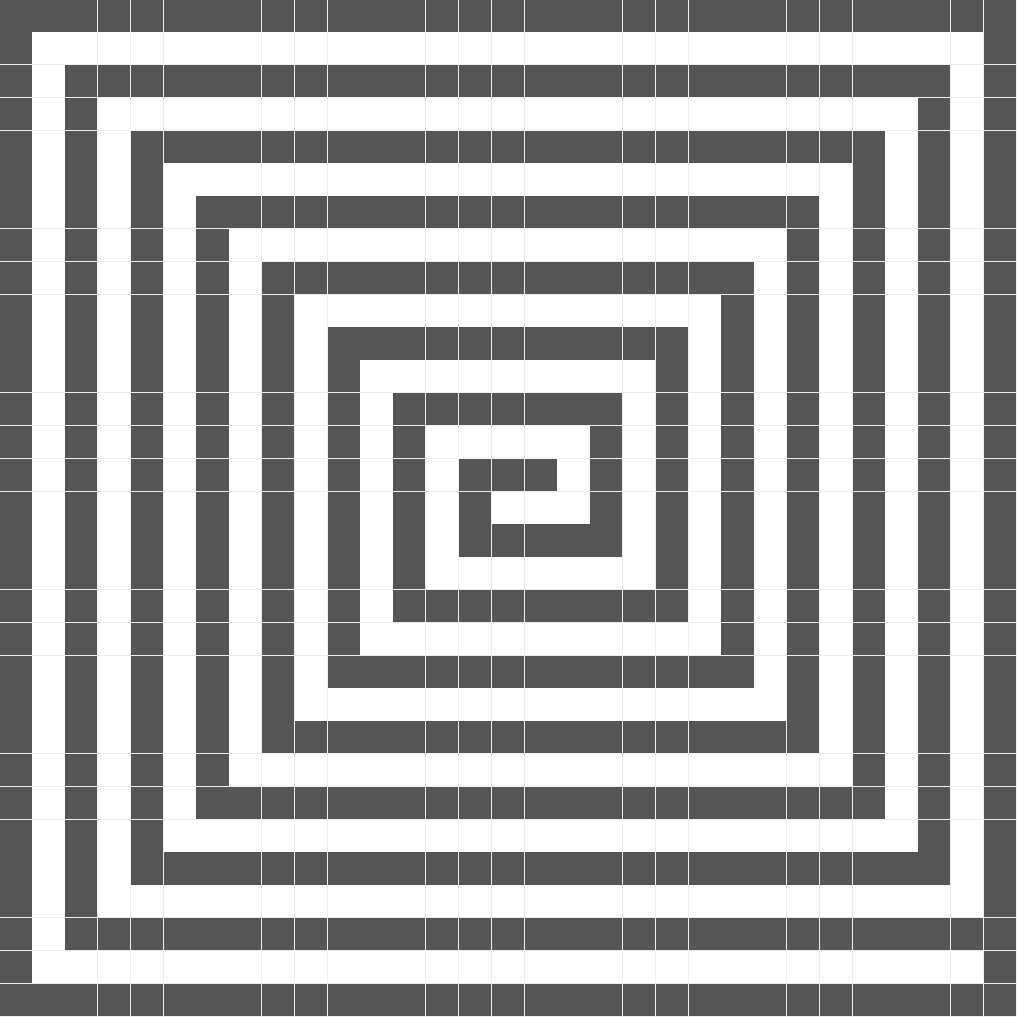
\includegraphics[width=.6\textwidth]{./immagini/mspirale.pdf}
  \caption{Una mappa a spirale con 7 avvolgimenti e intralcio medio di 12.9}
  \end{figure}
\subsection{Cattivi comportamenti}
  Su mappe che presentano una complessità elevata l'algoritmo simple può esibire
  comportamenti periodici. Facciamo qualche considerazione sul modello:
  \begin{itemize}
    \item lo stato dell'esplorazione è completamente definito dalla posizione
    degli agenti e dall'insieme delle celle, ciascuna nei 3 stati possibili per
    le celle
    \item lo stato successivo è derminato univocamente a partire dall'attuale
    \item il numero di celle è considerato finito
  \end{itemize}
  Da ciò segue che l'esplorazione può trovarsi in un numero finito di stati;
  questo ci assicura di non avere a che fare con un Halting Problem \cite{wiki:halting},
  e che anzi sicuramente, in presenza di un comportamento periodico, il sistema
  passerà più volte da uno stesso stato; ciò fornisce un metodo per poter rilevare
  con certezza tali comportamenti ciclici, seppure non di pratico utilizzo.
\subsection{Strumenti utilizzati}
  Per poter simulare e testare il modello è stato utilizzato il linguaggio
  Python unito con il framework mesa appositamente progettato per simulazioni
  multi-agente.
\subsection{Discrepanze implementative}
  A differenza di quanto descritto nel modello a livello implementativo la mappa
  è unica; tuttavia questo non modifica il comportamente descritto.
  Un'altra differenza tra modello e implementazione è il fatto che nel framework 
  i robot si muovono uno per volta mentre nel modello dovrebbero muoversi
  contemporaneamente. Tuttavia questa differenza dovrebbe essere vista come
  l'introduzione di una priorità di movimento necessaria nel caso di contese di
  una cella.

\newpage
\section{Algoritmi}
  Per poter analizzare il modello è stato necessario implementare alcuni algoritmi
che soddisfacessero due obiettivi fondamentali:
\begin{itemize}
  \item Ricerca dell'obiettivo
  \item Path finding
\end{itemize}

\subsection{Ricerca dell'obiettivo}
  Per selezionare il miglior obiettivo da raggiungere è stato progettato un algoritmo
  che seleziona la cella di bordo con il minor valore calcolato con la seguente
  equazione:
  $$target\_value = \delta(pos, border\_cell)^2 - \sum _{x \in other\_robot}{\delta(x,border\_cell)^2}$$
  dove le celle di bordo sono state definite come quelle celle che sono transitabili e che confinano con almeno una cella 
  non esplorata.
  Questa euristica tenta dunque di selezionare un obiettivo che sia vicino al robot in analisi e lontano dagli altri.
  Il concetto di "lontano" è stato implementato come distanza euclidea; questa scelta è molto efficiente a livello
  implementativo, tuttavia potrebbe risultare subottimale per quanto riguarda la scelta dei goal in quanto non tiene
  conto di possibili ostacoli durante il percorso.
  Per rendere più stabile la scelte di un goal e non farlo cambiare ad ogni tick, deve verificarsi una delle seguenti condizioni perché possa essere modificato:

  \begin{itemize}
    \item La cella selezionata non è più obiettivo in quanto qualcuno (anche il robot stesso) ha esplorato tutti 
          i suoi dintorni
    \item Viene trovato un obiettivo molto migliore; in questo caso la soglia di "testardaggine" del robot viene definita da un
        parametro che determina di quanto un obiettivo deve essere migliore di quello attuale per poterlo sostituire
  \end{itemize}
  \newpage
  \renewcommand{\fcolorbox}[4][]{#4}
  \inputminted[linenos,fontsize=\footnotesize]{python}{algoritmi/goal.py}
    Andiamo ora ad analizzare la complessità dell'argoritmo: Sia N il numero di 
    celle e A il numero di agenti:
    \begin{enumerate}
      \item Ricerca delle celle di frontiera; complessità $O(N)$
      \item Calcolo del punteggio di ogni cella rispetto all'agente; complessità $O(N\cdot A)$
    \end{enumerate}
    Di conseguenza possiamo dire che l'algoritmo per la ricerca dell'obiettivo ha complessità:
    $$O(N) + O(N \cdot A) = O(N \cdot A)$$
  \newpage
\subsection{Path finding}
  Il problema del path finding è un problema ampiamente trattato dalla letteratura sia
  dal punto di visto videoludico che da quello robotico; per questo motivo sono stati
  provati diversi algoritmi; alcuni suggeriti dalla letteratura mentre altri progettati da zero.
  
  Ogniqualvolta il "territorio" non è conosciuto a priori bisogna tener conto della
  necessità di ricalcolare il percorso quando viene scoperto un ostacolo; troviamo in
  \cite{ferguson2005guide} una descrizione dettagliata degli algoritmi di planning - replanning;
  inoltre gli algoritmi "anytime" permettono di raffinare nel tempo un path subottimale, e
  tale procedimento è applicabile ad A*. Tuttavia ciò non è presente nella nostra
  implementazione.
  \subsubsection{Algoritmo di Dijkstra}
    La mappa su cui si muovono i robot è una griglia ma può essere facilmente vista
    come un grafo dove ogni cella è un nodo connesso solo con le celle adiacenti. A questo
    punto è facile applicare l'algoritmo di Dijkstra per poter
    trovare un miglior percorso dalla posizione del robot fino all'obiettivo selezionato.
  \subsubsection{Algoritmo $A^*$}
  \label{complastar}
  L'algoritmo $A^*$ \cite{wiki:A*} è ben noto nel campo delle simulazioni ad agenti
  perché può sfruttare in maniera euristica la struttura spaziale della
  griglia: l'algoritmo si comporta come una ricerca depth-first sull'albero
  dei percorsi, ma dà la precedenza alla ricerca lungo i percorsi migliori
  secondo un'euristica specificabile; nel nostro caso utilizziamo la
  distanza euclidea.
  \inputminted[linenos,fontsize=\footnotesize]{python}{algoritmi/astar.py}
  Segue la struttura dello step che utilizza l'algoritmo $A*$.
  \inputminted[linenos,fontsize=\footnotesize]{python}{algoritmi/step_astar.py}
  La complessità dell'algoritmo $A^*$ nel caso peggiore è : $O(b^d)$ dove b è il numero di
  possibili successori per ogni cella e d è la lunghezza dello shortest path. 
  \newpage
  \subsubsection{Algoritmo greedy (simple)}
  \label{complgreedy}
    Questo algoritmo è stato progettato per essere di facile computazione; per questa ragione non calcola un path
    ma seleziona una mossa per volta utilizzando come metrica la distanza euclidea. Scegliendo ad ogni mossa
    la cella più libera più vicina però si richia di incorrere in loop che impediscono ad un robot di superare
    determinati ostacoli. Per questa ragione si è deciso di aggiunre come ulteriore clausola il fatto che fino a 
    quando un robot non cambia obiettivo non può passare due volte sulla stessa casella.
    Nel caso in cui però il robot non si possa più muovere perchè circondato da celle già percorse vengono rese
    nuovamente percorribili delle celle già percorse partendo da quelle più recenti e andando indietro; le celle vengono
    rese percorribili se hanno almeno un vicino percorribile.
    \inputminted[linenos, fontsize=\footnotesize]{python}{algoritmi/simple.py}
    La complessità di questo algoritmo dipende prevalentemente dal numero di celle già percorse; si potrebbe dunque
    dire che si tratta di un algoritmo a complessità : 
    \begin{itemize}
      \item $\Omega(1)$ nel caso migliore
      \item $O(s^2)$ nel caso peggiore  
    \end{itemize}
    dove s è il numero di celle già percorse durante il perseguimento dell'obiettivo attuale.
    

\newpage
\section{Risultati}
  \subsection{Misurazioni}
Per giudicare la bontà degli algoritmi sono state utilizzate varie mappe di 
diversa complessità (calcolata come in sezione \ref{mapcomplex}).
Per valutare i risultati abbiamo raccolto le seguenti misure:

\begin{itemize}
    \item Tempi medi di esplorazione (funzione del numero di robot)
    \item Efficienza media di esplorazione (funzione del tempo)
    \item Quantità media di comunicazione (funzione del tempo)
    \item La deviazione standard dei tempi ottenuti
    \item La regressione rispetto alla funzione $T(s) = (1-p)T + \frac{p}{s}T$
          dei valori dei tempi; forniamo il parametro $p$ e l'errore
          di regressione come deviazione standard dalla funzione ``fittata''.
\end{itemize}
\newcommand{\mapComplexity}[0]{}
\newcommand{\mapDescription}[0]{}
\newcommand{\nomeMappa}[0]{}
\newcommand{\pSimpleFit}[0]{}
\newcommand{\pAstarFit}[0]{}
\newcommand{\errSimpleFit}[0]{}
\newcommand{\errAstarFit}[0]{}


\foreach \s in { me, m1, m2, m3, mc} {
		%\newpage
    \input{sections/mappa_\s.tex}
    \subsection{\nomeMappa}

		\begin{figure}[H]
    		\includegraphics[width=1\textwidth]{presentaz/grafici/\s.pdf}
    		\caption{Questa mappa ha complessità \mapComplexity}
    	\end{figure}
    	
    	\mapDescription    	
    	
    	\begin{figure}[H]
          \centering
          \makebox[\textwidth][c]{
		  \subfloat[Tempi dell'algoritmo simple sulla \nomeMappa. ]{ 
			\shortstack{
		      \includegraphics[width=0.7\textwidth]{immagini/runall_\s_tempi_simple.pdf} \\
			  \small{Risultati del fit: $p = \pSimpleFit, std=\errSimpleFit$}}
			}
			\subfloat[Tempi dell'algoritmo $A*$ sulla \nomeMappa.]{
			\shortstack{
			  \includegraphics[width=0.7\textwidth]{immagini/runall_\s_tempi_astar.pdf} \\
			  \small{Risultati del fit: $p = \pAstarFit, std=\errAstarFit$}}
			}
		  }
		\end{figure}
		\begin{figure}[H]
    	  \makebox[\textwidth][c]{
		    \subfloat[Esplorazione della \nomeMappa]{
			  \includegraphics[width=0.7\textwidth]{immagini/runall_\s_espl.pdf}
			}
			\subfloat[Comunicazioni]{
			  \includegraphics[width=0.7\textwidth]{immagini/runall_\s_comun.pdf}
			}
	      }
		\end{figure}
		\begin{figure}[H]
    	  \centering
    	  \makebox[\textwidth][c]{
			\subfloat[Deviazione standard \nomeMappa]{ 
			  \includegraphics[width=0.7\textwidth]{immagini/runall_\s_std_tempi.pdf}
		    }
		  }
		\end{figure}
		
}

\subsection{Osservazioni sui risultati}
    Tutti i test sono stati svolti 5 volte per ogni possibile numero di agenti tra 1 e 20;
    tuttavia per l'algoritmo $A^*$ è stata utilizzato un valore di stubborness pari a
    0.5 mentre per l'algoritmo simple ne è stato utilizzato uno pari a 0.3; questa
    scelta deriva dal fatto che l'algoritmo simple essendo greedy entra con più facilità
    in loop con effetti quantomeno deleteri. Ciononostante è capitato, durante la
    campagna di simulazione, che alcune mappe causassero un loop nell'algoritmo simple. 
    

\newpage
\section{Conclusioni}
    I risultati sono generalmente coerenti con le aspettative; tuttavia particolari
conformazioni possono migliorare considerevolmente il comportamento
dell'algoritmo simple. Spesso i due algoritmi sono comparabili; tuttavia è bene
notare che la performance di $A*$ è probabilmente limitata dall'algoritmo per la 
scelta del goal, di natura greedy: infatti quest'ultimo non sfrutta
l'ottimalità del path calcolato da $A*$.

Nei risultati non è mai stata presa in considerazione la complessità degli
algoritmi come metrica, tuttavia, dato lo studio nelle sezioni \ref {complastar}
e \ref{complgreedy}, è chiaro che la scelta dell'algoritmo dovrebbe essere
influenzata dalla disponibilità di potenza computazionale dei singoli strumenti.

\subsection{Metrica di impedimento medio}
La metrica da noi sviluppata ha lo svantaggio di essere computazionalmente molto
onerosa, e di non predire fedelmente il comportamento del nostro algoritmo ``simple'';
tuttavia è anche da imputarsi dal fatto che tale algoritmo è solo parzialmente greedy,
in quanto l'accorgimento delle ``smelly cells'' gli conferisce maggior resistenza
contro i loop.

Sosteniamo tuttavia che la metrica sia effettivamente indicativa della difficoltà
di spostarsi sulla mappa con un algoritmo greedy, e più generalmente fornisca
una buona stima dell'aumento di lunghezza di un percorso dettata dalla topologia
della mappa.
\subsection{Possibili sviluppi futuri}
Sarebbe interessante caratterizzare con precisione la formazione dei
comportamenti periodici in relazione ai parametri di stubborness e della
complessità della mappa; inoltre si potrebbe ideare una metodologia di detection
e recovery dei loop, o comportamenti non del tutto deterministici volti a
renderne improbabile la formazione.

Un ambito di ulteriore sviluppo è la funzione di selezione del goal; un'euristica
che tenga maggior conto del territorio potrebbe aumentare l'efficienza
dell'esplorazione.

Se da un lato l'intero modello è stato pensato come simulazione software, ci si
può chiedere la fattibilità di un'implementazione hardware, e le sue caratteristiche;
il modello richiede un sistema di comunicazione robusto, di capacità che dipende
dal numero dei robot impiegati; inoltre la necessità di avere una comunicazione
broadcast costante tra i robot richiede un raggio di comunicazione almeno pari alla
distanza tra i 2 punti più lontani raggiungibili dagli agenti.
\newpage
\nocite{*}
 \printbibliography

\end{document}
